\documentclass[12pt]{article}
\usepackage[utf8]{inputenc}
\usepackage[]{multicol}
\usepackage[auth-lg]{authblk}
\usepackage[margin=1.2in]{geometry}
\usepackage[]{graphicx}
\usepackage[]{ctable}
\usepackage[]{natbib}
\usepackage[]{array}
\newcolumntype{P}[1]{>{\centering\arraybackslash}p{#1}}

\title{Benchmarking Current RNA Folding Software and Improvements to the Current Regime}

\begin{document}
\author{Jianglin Liu}
\author{Bingxi Li}
\author{Gregory Rehm}
\affil{\normalsize{University of California, Davis}
\{\texttt{jiliu, bxli, grehm\}@ucdavis.edu}}
\maketitle

\begin{abstract}
Finding the secondary structure of RNA is important for understanding how RNA
will interact in a cell. Frequently computational algorithms are used to determine
structure due to difficulties extracting good \textit{in vivo} data of RNA
structures. Many of the algorithms for RNA folding are computationally complex.
In this paper we establish benchmarks for two commonly used RNA folding packages,
mfold, and RNAfold Vienna, and compare them to an improved Four-Russians folding
algorithm. We show ... These results will help software maintainers to understand
the benefit of updating their algorithms. The results will also help guide users
when choosing RNA folding software when looking for the most computationally optimal package.
\end{abstract}
\section{Introduction}
\par RNA is an essential macromolecule used in protein formation and performs
other essential functions within the body\cite{turner}. RNA does not stay in
single stranded form and instead folds on itself to create the lowest energy
conformation possible to ensure thermodynamic stability\cite{herschlag}. When
folding, RNA forms a 2D secondary structure\cite{mccaskill} with A matching to U
and G to C (figure 1).  Using this data we can find a 3D tertiary structure\cite{mccaskill}.
\begin{figure}[ht!]
  \centering
  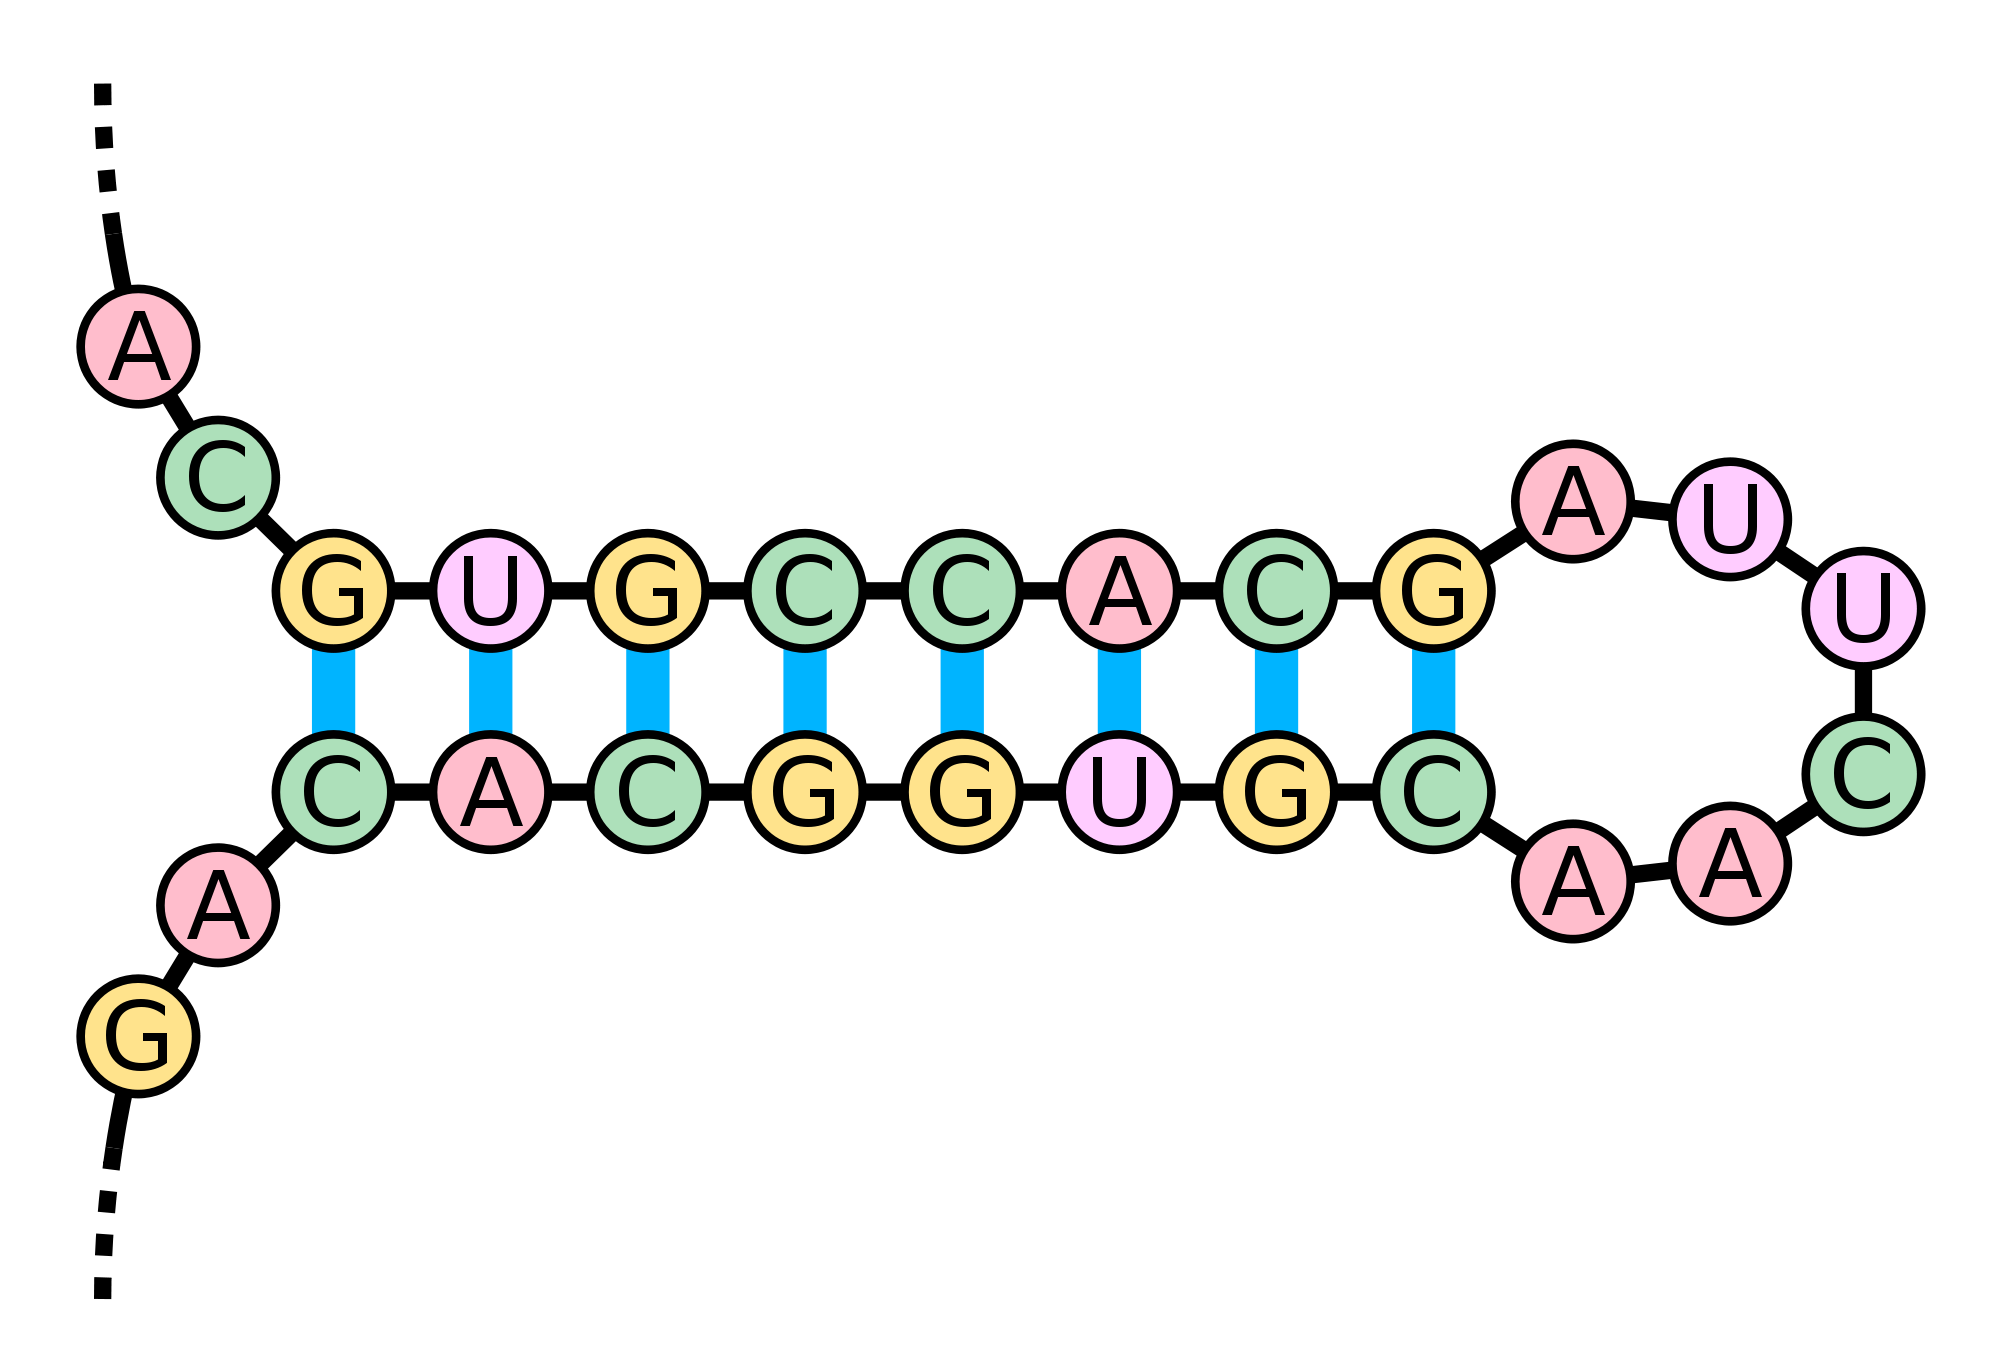
\includegraphics[keepaspectratio, scale=0.12]{fold-example.png}
  \caption{Example of an RNA molecule folding}
  \label{fig:RNA Folding}
\end{figure}
\par Our paper focuses on benchmarking 2D secondary structure prediction software
based off the Nussinov dynamic programming algorithm\cite{nussinov} for RNA folding.
This algorithm is $O(n^3)$ time complexity. There have been multiple attempts to
parallelize the Nussinov algorithm\cite{rizk, other-gpu} which have resulted in
large speed increases, however, CPU intensive algorithms only slightly lowered
the bound up until 2010\cite{minor-nussinov-improvement, chan}. In 2010 the
Nussinov bound that was significantly improved by the Frid-Gusfield Four Russians
method which established you could perform the DP method in $O(\frac{n^3}{log(n)})$
time\cite{gusfield}. Later a parallel method of the Four Russians algorithm
presented proof that you can lower this bound to $O(\frac{n^2}{log(n)})$ inside
an NVIDIA CUDA environment\cite{balaji}.
\par There are two major RNA folding software packages, mfold\cite{zuker1989,zuker1981},
and the Vienna RNA Package\cite{vienna}. These both utilize the Nussimov method
to return results of the RNA secondary structure by finding the lowest possible
thermodynamic conformations of the RNA\cite{zuker1981,vienna}. In order to tell
which was faster we performed application level benchmarks\cite{eulogy} to see
which of these two applications could more quickly fold arbitrary length RNA of
the circular and linear variety. The way mfold is written allows linear RNA to
be treated as exceptional variants of circular ones\cite{circular}. RNAfold
Vienna was initially optimized to only handle linear RNA\cite{circular} but
later improvements enabled it to speed the folding of circular ones\cite{circular}.
As a result we also wish to determine what kind of speed difference still exists
between mfold and Vienna when performing analysis on circular RNA.

\par We then performed micro-benchmarks\cite{sysperformance} of the folding
algorithms utilized in mfold and Vienna for both circular and linear RNA, and
then compared that to equivalent benchmarks for the Four Russians and parallel
Four Russians algorithms. The first thing we found when comparing mfold and
Vienna was ... . When we compared mfold and Vienna to the Four Russians algorithms
we found that without a graphics card and parallel processing capabilities a
machine can see speed ups of ... in mfold and ... in Vienna for linear RNA. For
circular RNA speed increases change to ... in mfold and ... in Vienna. With a
graphics card and parallel processing folding clusters can see increases of up
to ... for mfold and ... in Vienna. Circular RNA also sees speed bumps of ... in
mfold and ... in Vienna.
\par These results show us that ... for natively differentiating between mfold
and Vienna. They also help explain that both pieces of software can experience
significant speed increases if they implemented the Frid-Gusfield method. Furthermore
the authors of this paper would recommend both software packages to support GPU
hardware to achieve even greater speed gains when inside a parallel capable
environment.

\section{Methods}
\subsection{Standardizing the Testing Environment}
Benchmarking is renown as a difficult thing to perform effectively\cite{sysperformance,eulogy}.
There are many processes that can be executing on a computer at any one moment
that it is possible that a benchmark can give inaccurate information due to
conflicting processes running in the background\cite{sysperformance}. As a result
we used a machine solely dedicated for benchmarking and no other tasks. We also
standardized on the following specifications for our runs\cite{benchspecs}:
\begin{center}
    \begin{tabular}{P{5.0cm}P{3.5cm}P{3.0cm}}
        \specialrule{.1em}{.05em}{.05em}
        \textbf{Architecture} & \textbf{Operating System} & \textbf{Compiler} \\ \hline
        8 core Intel i7 CPU 4.00 GHz 16G RAM GeForce GTX 960 & Linux 4.2.5-201 Fedora 22 & GCC 5.1.1-4.fc22 \\ \hline
        " & " & gcc-gfortran 5.1.1-4.fc22\\ \hline
        " & " & NVIDIA CUDA version 5.5 \\
        \specialrule{.1em}{.05em}{.05em}
    \end{tabular}
\end{center}
We used the following applications with corresponding versions and requirements in our test runs:
\begin{center}
    \begin{tabular}{ccc}
        \specialrule{.1em}{.05em}{.05em}
        \textbf{Application} & \textbf{Version} & \textbf{Requirements} \\ \hline
        mfold & 3.6 & GCC, Fortran \\ \hline
        RNAfold Vienna  & 2.1.9 & GCC \\ \hline
        Frid-Gusfield Four Russians & N/A & GCC \\ \hline
        Parallel Four Russians & N/A & GCC, NVIDIA CUDA \\
        \specialrule{.1em}{.05em}{.05em}
    \end{tabular}
\end{center}
\par Our testing architecture was laid out where we would SSH into the benchmarking
machine and then execute tests. Test results would then be reported back to the
user's central machine where they could be stored in a database for later analysis
(figure 2). Our testing required no internet connectivity besides the ssh access
required to initiate our testing so all calculations were performed locally. Also
there were no IO operations except for post processing of mfold and Vienna results.
\begin{figure}[ht!]
  \centering
  \includegraphics[keepaspectratio, scale=0.7]{benchmarking-architecture.png}
  \caption{Test Architecture}
  \label{fig:Testing Arch}
\end{figure}

\subsection{Data Inputs}
\par For input data we give inputs of RNA as strings in a file. An example of this
would be the 10 character RNA string AUGCCAUGGA. This same RNA sequence can be
treated as circular by providing parameters to the mfold and RNAfold Vienna
programs that tell it the RNA is circular\cite{mfold-manual, vienna-manual}.
\subsection{Application Benchmarks}
\par The first type of benchmark we perform is the application level benchmark.
An application benchmark is designed to measure the performance of an entire
application and the resources it consumes on an individual machine\cite{jain}.
In our case we wish to evaluate the amount of time that mfold and RNAfold Vienna
take to return RNA secondary structures given different length RNA strands varying
on linear and circular variety. Since a single run of an application may vary in
time even for identical inputs. Because of this we evaluate each input of RNA 30
times and report the mean $\mu$, standard deviation, $\sigma^2$, of the runs
corresponding to each sequence length.

\subsection{Micro-benchmarks}
\par The most basic type of benchmark to perform is the micro-benchmark. The
micro-benchmark is a single piece of code executed many times in serial so that
we can get a profile of its run characteristics\cite{eulogy,sysperformance}.
Once these characteristics are observed we can then make inferences about its
performance and ways that it can be improved. Micro-benchmarks have the downside
of losing generality of performance across the entire application\cite{eulogy, sysperformance}.
A good example of this is if an IO heavy function made many consecutive calls to
the \textit{read} function on the OS while the rest of the application made no
calls to \textit{read} whatsoever. If we tried to generalize this one function to
the rest of the application we would misguidedly attempt to optimize disk IO
across our entire system.
\par We avoid this trap in our paper by benchmarking only parts of the code that
execute the Nussinov algorithm in mfold and the Vienna package. We then report
these results back to our test results database for later analysis. After this we
compare these results to runs of the serial Frid-Gusfield algorithm and parallel
Frid-Gusfield algorithm.

\subsection{Frid-Gusfield Four-Russians Algorithm}
\par The Four-Russians Algorithm \cite{gusfield} is an algorithm to improve the above-mentioned Nussinov $O(n^3)$ Algorithm by Four-Russian method. The Frid and Gusfield is an $O(\frac{n^3}{\log n})$ algorithm.
\par The Four Russian algorithm achieves this speed up by understanding that we can make certain optimizations to the matrix of matching base pairs required by the Nussinov algorithm. Particularly, the values along a column from bottom to top and along a row from left to right are monotonically non-decreasing. Consecutive cells differ at most by 1\cite{gusfield}. As a result we can perform pre-processing of specific operations that the Nussinov algorithm must compute manually.

\par The Four-Russians Algorithm \cite{gusfield} is a two-vector algorithm to
improve the above-mentioned Nussinov $O(n^3)$ Algorithm. The Frid and Gusfield
is an $O(\frac{n^3}{\log n})$ algorithm. The Four Russian algorithm achieves
this speed up by understanding that we can make certain optimizations to the
matrix of matching base pairs required by the Nussinov algorithm. Particularly,
the values along a column from bottom to top and along a row from left to right
are monotonically non-decreasing. Consecutive cells differ at most by 1\cite{gusfield}.
As a result we can perform pre-processing of specific operations that the
Nussinov algorithm must compute manually.

\subsection{CUDA Parallel Implementation for F-G Method}
\par Compute Unified Device Architecture (CUDA) is a parallel computing platform created by NVIDIA. By using CUDA API, Venkatachalam presented an $O(\frac{n^2}{logn})$ algorithm for RNA folding is presented \cite{balaji}. The CUDA implementation parallelizes the two-vector method so that achieve an enhancement of another factor of $O(n)$.

\section{Results}

\subsection{Application Benchmarks}
In this part, we performed the benchmark for two packages under Dynamic Programing (DP) paradigm with both linear and circular RNA. The packages that we are interested in are \textit{Vienna Package} \cite{vienna} and \textit{m-fold Package} \cite{zuker1989,zuker1981}. And their capacities to predict the secondary structure of RNA are tested with two types of RNA at different length.

For the benchmark of linear type of RNA, we select the RNA of the size, ranging from 200 nucleotides to 1000 nucleotides. The test is performed for 30 times for each size in order to derive the mean time and standard deviation. The time to fold these structures are compared in the following Table 1.
\begin{table}[h!]
    \begin{tabular}{ |p{1.5cm}||p{1.2cm}|p{1.2cm}|p{1.2cm}|p{1.2cm}|p{1.2cm}|p{1.2cm}|p{1.2cm}| p{1.2cm} | p{1.2cm} |}
    \hline
    \multicolumn{10}{|c|}{Timing of $m-fold$ for linear RNA (sec.)} \\
    \hline
    Size& 200& 300& 400& 500& 600& 700 & 800 & 900 & 1000\\
    \hline
    N runs& 30 & 30& 30 & 30& 30& 30& 30& 30& 30\\
    \hline
    average& 2.523 & 6.635 & 6.313 & 8.336 & 10.492 & 9.384 & 12.212 & 14.319 & 14.402\\
    std ($\sigma^2$) &0.343 & 0.251 & 0.180 & 0.547 & 0.144 & 0.094 & 0.176 & 0.118 & 0.211 \\
    \hline
    \end{tabular}

    \begin{tabular}{ |p{1.5cm}||p{1.2cm}|p{1.2cm}|p{1.2cm}|p{1.2cm}|p{1.2cm}|p{1.2cm}|p{1.2cm}| p{1.2cm} | p{1.2cm} |}
    \hline
    \multicolumn{10}{|c|}{Timing of $Vienna$ for linear RNA (sec.)} \\
    \hline
    Size& 200& 300& 400& 500& 600& 700 & 800 & 900 & 1000\\
    \hline
    N runs& 30 & 30& 30 & 30& 30& 30& 30& 30& 30\\
    \hline
    average& 0.029 & 0.072 & 0.112 & 0.163 & 0.508 & 0.491 & 1.934 & 11.723 & 8.296\\
    std ($\sigma^2$) &0.006 & 0.001 & 0.001 & 0.001 & 0.002 & 0.002 & 0.006 & 0.336 & 0.011 \\
    \hline
    \end{tabular}
\caption{The time taken by two packages to predict secondary structures of linear RNA of different length.}
\end{table}

In a more vivid way, the plot of the bechmark time for linear RNA are shown in the Fig 3.\\
\begin{figure}[htbp!]
    \centering
    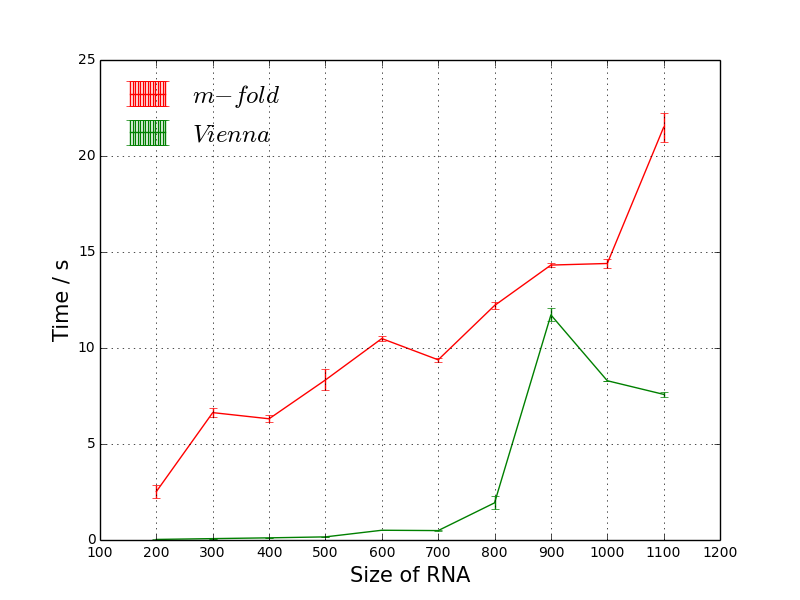
\includegraphics[width=0.75\textwidth]{l-m-v.png}
    \caption{Benchmark of $Vienna$ and $m-fold$ packages with linear RNA of different sizes.}
\end{figure}

When the size of RNA is within 1000 nucleotides, the $Vienna$ packages is more efficient than the $m-fold$ package. But the $Vienna$ package increases faster than the $m-fold$ package. Probably, the $Vienna$ Package is not advantageous to predict the secondary structure of super large RNA.

Moreover, the benchmark circular type of RNA is also performed here. In this test, the size of the RNA is between 200 nucleotides to 1000 nucleotides. The time in seconds to determine their secondary structures are listed in the following Table 2.

\begin{table}[h!]
\begin{center}
\begin{tabular}{ |p{1.5cm}||p{1.2cm}|p{1.2cm}|p{1.2cm}|p{1.2cm}|p{1.2cm}|p{1.2cm}|p{1.2cm}| p{1.2cm} | p{1.2cm} |}
\hline
\multicolumn{10}{|c|}{Timing of $m-fold$ for circular RNA (sec.)} \\
\hline
Size& 200& 300& 400& 500& 600& 700 & 800 & 900 & 1000\\
\hline
N runs& 30 & 30& 30 & 30& 30& 30& 30& 30& 30\\
\hline
average& 2.409 & 6.633 & 6.269 & 8.889 & 11.274 & 9.074 & 11.358 & 14.678 &16.712\\
std ($\sigma^2$) & 0.060 & 0.354 & 0.362 & 0.159 & 0.1176 & 0.161 & 0.364 & 0.1999 & 0.285 \\
\hline
\end{tabular}
\begin{tabular}{ |p{1.5cm}||p{1.2cm}|p{1.2cm}|p{1.2cm}|p{1.2cm}|p{1.2cm}|p{1.2cm}|p{1.2cm}| p{1.2cm} | p{1.2cm} |}
\hline
\multicolumn{10}{|c|}{Timing of $Vienna$ for circular RNA (sec.)} \\
\hline
Size& 200& 300& 400& 500& 600& 700 & 800 & 900 & 1000\\
\hline
N runs& 30 & 30& 30 & 30& 30& 30& 30& 30& 30\\
\hline
average& 0.027 & 0.084 & 0.129 & 0.153 & 0.664 & 0.351 & 1.943 & 7.915 & 50.15\\
std ($\sigma^2$) & 0.002 & 0.001 & 0.001 & 0.002 & 0.002 & 0.002 & 0.006 & 0.036 & 0.126 \\
\hline
\end{tabular}
\end{center}
\caption{The time taken by two packages to predict secondary structures of circular RNA of different length.}
\end{table}

The following Fig 4 is plotted to better visualize how the two packages compete with each other. The $Vienna$ can do a more efficient prediction when the circular RNA has nucleotides smaller than 950. As the operations required for $Vienna$ prediction increases rapidly for RNA longer than 900 nucleotides, the $Vienna$ package loses its advantages. And the $m-fold$ package demonstrates better performance.

\begin{figure}[htbp!]
\centering
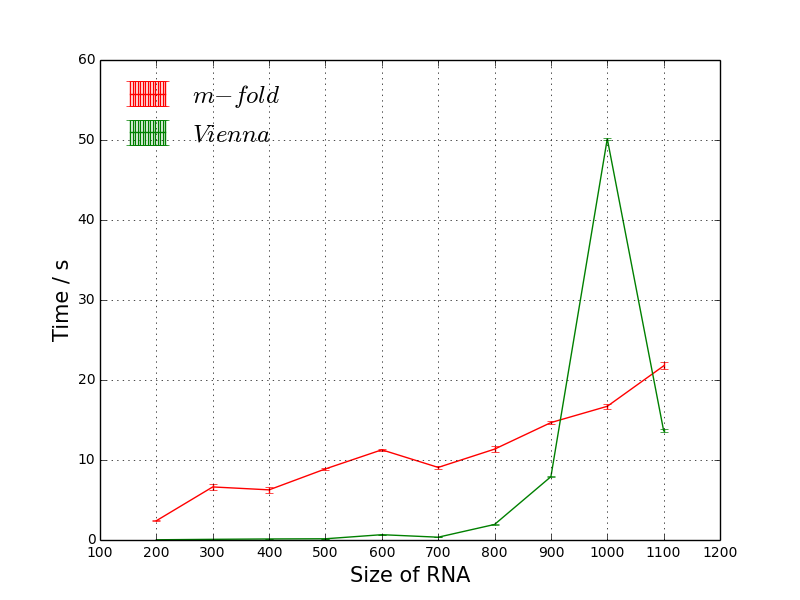
\includegraphics[width=0.75\textwidth]{c-m-v.png}
\caption{Benchmark of $Vienna$ and $m-fold$ packages with circular RNA of different sizes.}
\end{figure}

Through the above benchmark analysis, we have developed a clear insight into the performance of two packages, $Vienna$ and $m-fold$ packages. Linear and circular types of RNA have been well tested at several length. In both of the cases, the $Vienna$ packages is time-optimal for small RNA no larger than 900 nucleotides. However, this package loses its advantages to $m-fold$ after 1000 nucleotides.

\subsection{Micro-benchmarks}
The timing for Nussinov, FG and CUDA Four-Russian algorithms are listed below with different sizes of RNA sequences.\\
\begin{center}
    \begin{tabular}{ |p{1.5cm}||p{1.2cm}|p{1.3cm}|p{1.3cm}|p{1.4cm}|p{1.4cm}|p{1.4cm}|p{1.6cm}|}
     \hline
     \multicolumn{8}{|c|}{Timing of Algorithms for RNA Folding (sec.)} \\
     \hline
     Size& 500& 1000& 2000& 3000& 4000& 5000& 6000\\
     \hline
     Nussinov& 0.2790& 2.0751& 16.7033& 57.8146& 145.2998& 301.4874& 519.6531\\
     Frid-Gusfield& 0.0903& 0.6092& 5.5868& 19.6117& 49.3309& 95.6461& 162.9072\\
     CUDA& 0.0088& 0.1988& 0.4690& 1.1943& 2.5817& 4.8506& 8.2735\\
     \hline
    \end{tabular}
\end{center}\\
\\
\\
The data are plotted visually as below:
\begin{figure}[ht!]
  \centering
  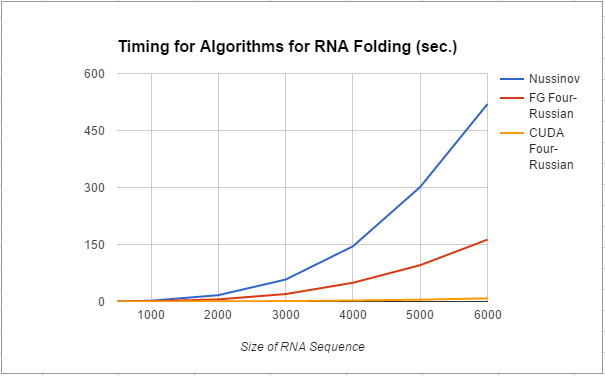
\includegraphics[keepaspectratio, scale=.92]{algorithmGraph.png}
  \caption{Timing of Algorithms for RNA Folding (sec.)}
  \label{fig:Timing_Algorithm}
\end{figure}

\section{Discussion}
In this paper, we performed both application and micro benchmark for current packages and some popular methods available for RNA secondary structure prediction problem, namely, RNA folding.

For application benchmark, $Vienna$ and $m-fold$ has been applied to predict two types of RNA. In both linear and circular cases, the $Vienna$ package has better performance while the $m-fold$ is time optimal in the prediction of RNA larger than 1000 nucleotides. However, this conclusion can be further confirmed by testing more $RNA$ sequences at the same length. Although the two packages are all based on Dynamical Programming paradigm, their average performance may be different. The difference might come from the ways how they implement the DP algorithm. For example, the code used for packages and the I/O management are probably the main reasons for this difference.

\begin{thebibliography}{56}
\bibitem{gusfield}
Frid Y, Gusfield D.
\textit{A simple, practical and complete O($n^3$)-time
algorithm for RNA folding using the Four-Russians Speedup}.
Algorithms Mol Biol 2010, 5:13

\bibitem{balaji}
Venkatachalam B, Gusfield D.
\textit{Faster algorithms for RNA-folding using the Four-Russians method}.
Algorithms for Molecular Biology20149:5.

\bibitem{nussinov}
Nussinov R, Jacobson A.
\textit{Fast algorithm for predicting the secondary structure of
single-stranded RNA}.
Proc. Nati. Acad. Sci. USA Vol. 77, No. 11, pp. 6309-6313, November 1980.

\bibitem{turner}
Mathews D, Turner D.
\textit{Prediction of RNA secondary structure by free energy
minimization}.
Current Opinion in Structural Biology 2006, 16:270–278.

\bibitem{mccaskill}
McCaskill J.S.
\textit{The Equilibrium Partition Function and Base Pair
Binding Probabilities for RNA Secondary Structure.}
Biopolymers, Vol. 29,1105-1119 (1990)

\bibitem{herschlag}
Herschlag D.
\textit{RNA Chaperones and the RNA Folding Problem}.
Vol. 270, No. 36, Issue of September 8, pp. 20871–20874, 1995

\bibitem{vienna}
Hofacker I. L, Fontana W, Stadler P. F, Bonhoeffer L. S, Tacker M, Schuster P.
\textit{Fast Folding and Comparison of RNA Secondary Structures}.
Monatshefte ftir Chemie 125, 167-188 (1994)

\bibitem{zuker1989}
Zuker M.
\textit{Computer Prediction of RNA Structure}.
Methods in Enzymology, vol. 180.

\bibitem{zuker1981}
Zuker M, Steigler P.
\textit{Optimal computer folding of large RNA sequences using thermodynamics and auxiliary information}.
Nucleic Acids Research vol. 9 Number 11981.

\bibitem{sysperformance}
Gregg B.
\textit{Systems Performance; Enterprise and the Cloud}.
Pearson Education 2014 Upper Saddle River, NJ

\bibitem{benchspecs}
Altun, O.
\textit{Clustering Application Benchmark}.
IISWC.2006.302742

\bibitem{minor-nussinov-improvement}
Akutsu, T.
\textit{Approximation and Exact Algorithms for RNA
Secondary Structure Prediction and Recognition
of Stochastic Context-free Languages}
Journal of Combinatorial Optimization 3, 321–336 (1999)

\bibitem{chan}
Chan TM.
\textit{More Algorithms for All-Pairs Shortest Paths in Weighted
Graphs}.
SIAM J Comput 2010, 39(5):2075-2089

\bibitem{eulogy}
Cantrill B.
\textit{Eulogy for a benchmark}.
The Observation Deck Web. http://dtrace.org/blogs/bmc/2009/02/02/eulogy-for-a-benchmark/.
2009.

\bibitem{rizk}
Rizk G, Lavenier D.
\textit{GPU accelerated Rna folding algorithm}.
Allen, G.; Nabrzyski, J.; Seidel, E.; Albada, G.D. van; Dongarra, J.; Sloot, P.M.A. 9th International Conference on Computational Science, May 2009, Baton Rouge, United States. Springer., 5544, pp.1031, 2009, LNCS. <10.1000.ISBN: 978-3-642-01969-2>. <hal-00425543>

\bibitem{other-gpu}
Chang D, Kimmer C, Ming O.
\textit{Accelerating the Nussinov RNA Folding Algorithm with CUDA/GPU}
Signal Processing and Information Technology (ISSPIT), 2010 IEEE International Symposium on, 15-18 Dec. 2010, pp. 120-125

\bibitem{circular}
Hofacker I, Stadler P.
\textit{Memory efficient folding algorithms for circular RNA secondary structures}.
Bioinformatics (2006) 22 (10): 1172-1176.

\bibitem{mfold-manual}
Zuker M, Matthews D.H, Turner D.H.
\textit{Algorithms and Thermodynamics for RNA
Secondary Structure Prediction:
a Practical Guide}.
The mfold Web Server Web. http://unafold.rna.albany.edu/doc/mfold-manual/mfold-3.0-manual.pdf.gz.

\bibitem{vienna-manual}
Hofacker I, Fontana W, Bonhoeffer S, Stadler P.F, Lorenz R.
\textit{RNAFOLD}.
Theoretical Biochemistry Group Institute for Theoretical Chemistry Web. https://www.tbi.univie.ac.at/RNA/RNAfold.1.html\#heading5

\bibitem{jain}
Jain, R.
\textit{Art of Computer Systems Performance Analysis Techniques For Experimental Design Measurements Simulation And Modeling}.
Wiley Computer Publishing, John Wiley \& Sons, Inc.
ISBN: 0471503363 Pub Date: 05/01/91.

\end{thebibliography}

\end{document}
